\item {\bf Linear Classifiers (logistic regression and GDA)}

In this problem, we cover two probabilistic linear classifiers we have covered in class so far. First, a discriminative linear classifier: logistic regression. Second, a generative linear classifier: Gaussian discriminant analysis (GDA). Both the algorithms find a linear decision boundary that separates the data into two classes, but make different assumptions. Our goal in this problem is to get a deeper understanding of the similarities and differences (and, strengths and weaknesses) of these two algorithms.

For this problem, we will consider two datasets, along with starter codes provided in the following files:
\begin{center}
\begin{itemize}
	\item \texttt{src-linearclass/ds1\_{train,valid}.csv}
	\item \texttt{src-linearclass/ds2\_{train,valid}.csv}
  \item \texttt{src-linearclass/submission.py}
\end{itemize}
\end{center}
Each file contains $\nexp$ examples, one example $(x^{(i)}, y^{(i)})$ per row. In particular, the $i$-th row contains columns $x^{(i)}_0\in\Re$, $x^{(i)}_1\in\Re$, and $y^{(i)}\in\{0, 1\}$. In the subproblems that follow, we will investigate using logistic regression and Gaussian discriminant analysis (GDA) to perform binary classification on these two datasets.

\begin{enumerate}
	\item \points{1a}

In lecture we saw the average empirical loss for logistic regression:
\begin{equation*}
	J(\theta)
	= -\frac{1}{\nexp} \sum_{i=1}^\nexp \left(y^{(i)}\log(h_{\theta}(x^{(i)}))
		+  (1 - y^{(i)})\log(1 - h_{\theta}(x^{(i)}))\right),
\end{equation*}
where $y^{(i)} \in \{0, 1\}$, $h_\theta(x) = g(\theta^T x)$ and $g(z) = 1 / (1 + e^{-z})$.

Find the Hessian $H$ of this function, and show that for any vector $z$, it holds true that
%
\begin{equation*}
  z^T H z \ge 0.
\end{equation*}
%
{\bf Hint:} You may want to start by showing that $\sum_i\sum_j z_i x_i x_j z_j = (x^Tz)^2 \geq 0$. Recall also that $g'(z) = g(z)(1-g(z))$.

{\bf Remark:} This is one of the standard ways of showing that the matrix $H$ is positive semi-definite, written ``$H \succeq 0$.''  This implies that $J$ is convex, and has no local minima other than the global one. If you have some other way of showing $H \succeq 0$, you're also welcome to use your method instead of the one above.\clearpage
	\item \points{1b}
Follow the instructions in \texttt{src/submission.py} to train a logistic regression classifier using Newton's Method. You will complete the |fit| and |predict| functions of the |LogisticRegression| class.

Starting with $\theta = \vec{0}$, run Newton's Method until the updates to $\theta$ are small: Specifically,  train until the first iteration $k$ such that $\vert\theta_{k} - \theta_{k-1}\vert_1 < \epsilon$, where $\epsilon = 1\times 10^{-5}$. Make sure to write your model's predicted probabilities on the validation set to the file specified in the code.

To verify a correct implementation, run the autograder test case |1b-4-basic| to create a plot of the \textbf{validation data} with $x_1$ on the horizontal axis and $x_2$ on the vertical axis. This plot uses a different symbol for examples $x^{(i)}$ with $y^{(i)} = 0$ than for those with $y^{(i)} = 1$. On the same figure, it will also plot the decision boundary found by logistic regression (i.e, line corresponding to $p(y\vert x) = 0.5$).

The output plot should look similar to the following (no plot submission is required): 

\begin{figure}[H]
	\centering
	\vspace{2mm}
	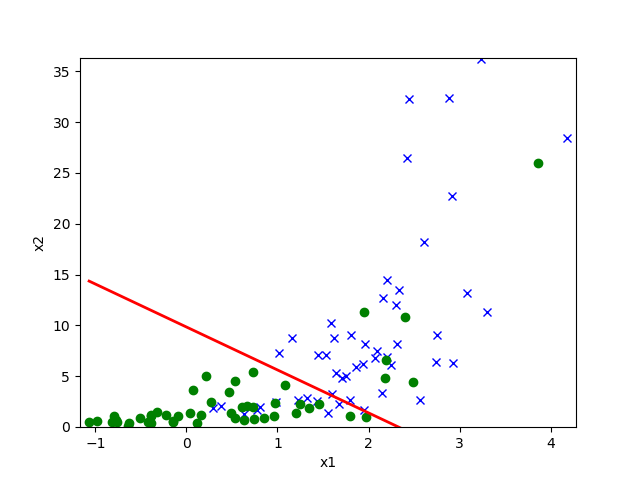
\includegraphics[width=0.65\linewidth]{01-linearclass/p01b_pred_1.png}
    \caption{Separating hyperplane for logistic regression on validation set of Dataset 1 (Note: This is for reference only.  You are not required to submit a plot.)}
\end{figure}

	\item \points{1c}
Recall that in GDA we model the joint distribution of $(x, y)$ by the following
equations:

\begin{eqnarray*}
	p(y) &=& \begin{cases}
	\phi & \mbox{if~} y = 1 \\
	1 - \phi & \mbox{if~} y = 0 \end{cases} \\
	p(x \vert  y=0) &=& \frac{1}{(2\pi)^{\di/2} \vert \Sigma\vert ^{1/2}}
		\exp\left(-\frac{1}{2}(x-\mu_{0})^T \Sigma^{-1} (x-\mu_{0})\right) \\
	p(x \vert  y=1) &=& \frac{1}{(2\pi)^{\di/2} \vert \Sigma\vert ^{1/2}}
		\exp\left(-\frac{1}{2}(x-\mu_1)^T \Sigma^{-1} (x-\mu_1) \right),
\end{eqnarray*}

where $\phi$, $\mu_0$, $\mu_1$, and $\Sigma$ are the parameters of our model.

Suppose we have already fit $\phi$, $\mu_0$, $\mu_1$, and $\Sigma$, and now
want to predict $y$ given a new point $x$. To show that GDA results in a
classifier that has a linear decision boundary, show the posterior distribution
can be written as

\begin{equation*}
	p(y = 1\mid x; \phi, \mu_0, \mu_1, \Sigma)
	= \frac{1}{1 + \exp(-(\theta^T x + \theta_0))},
\end{equation*}

where $\theta\in\Re^\di$ and $\theta_{0}\in\Re$ are appropriate functions of
$\phi$, $\Sigma$, $\mu_0$, and $\mu_1$.\\

	\item \points{1d}
Given the dataset, we claim that the maximum likelihood estimates of the parameters are given by
\begin{eqnarray*}
    \phi &=& \frac{1}{\nexp} \sum_{i=1}^\nexp 1\{y^{(i)} = 1\} \\
    \mu_{0} &=& \frac{\sum_{i=1}^\nexp 1\{y^{(i)} = {0}\} x^{(i)}}{\sum_{i=1}^\nexp 1\{y^{(i)} = {0}\}} \\
    \mu_1 &=& \frac{\sum_{i=1}^\nexp 1\{y^{(i)} = 1\} x^{(i)}}{\sum_{i=1}^\nexp 1\{y^{(i)} = 1\}} \\
    \Sigma &=& \frac{1}{\nexp} \sum_{i=1}^\nexp (x^{(i)} - \mu_{y^{(i)}}) (x^{(i)} - \mu_{y^{(i)}})^T
\end{eqnarray*}
The log-likelihood of the data is
\begin{eqnarray*}
    \ell(\phi, \mu_{0}, \mu_1, \Sigma) &=& \log \prod_{i=1}^\nexp p(x^{(i)} , y^{(i)}; \phi, \mu_{0}, \mu_1, \Sigma) \\
    &=& \log \prod_{i=1}^\nexp p(x^{(i)} \vert  y^{(i)}; \mu_{0}, \mu_1, \Sigma) p(y^{(i)}; \phi).
\end{eqnarray*}
By maximizing $\ell$ with respect to the four parameters, prove that the maximum likelihood estimates of $\phi$, $\mu_{0}, \mu_1$, and $\Sigma$ are indeed as given in the formulas above.  (You may assume that there is at least one positive and one negative example, so that the denominators in the definitions of $\mu_{0}$ and $\mu_1$ above are non-zero.)

	\item \points{1e}
In \texttt{src/01-linearclass/gda.py}, fill in the code to calculate $\phi$, $\mu_{0}$, $\mu_{1}$, and $\Sigma$, use these parameters to derive $\theta$, and use the resulting GDA model to make predictions on the validation set. Make sure to write your model's predictions on the validation set to the file specified in the code.

To verify a correct implementation, consider creating a plot of the \textbf{validation data} with $x_1$ on the horizontal axis and $x_2$ on the vertical axis. To visualize the two classes, use a different symbol for examples $x^{(i)}$ with $y^{(i)} = 0$ than for those with $y^{(i)} = 1$. On the same figure, plot the decision boundary found by GDA (i.e, line corresponding to $p(y\vert x) = 0.5$).\\

Please run GDA on dataset 1. No plot submission required. Your plot should look similar to the following:

\begin{figure}[H]
	\centering
	\vspace{2mm}
	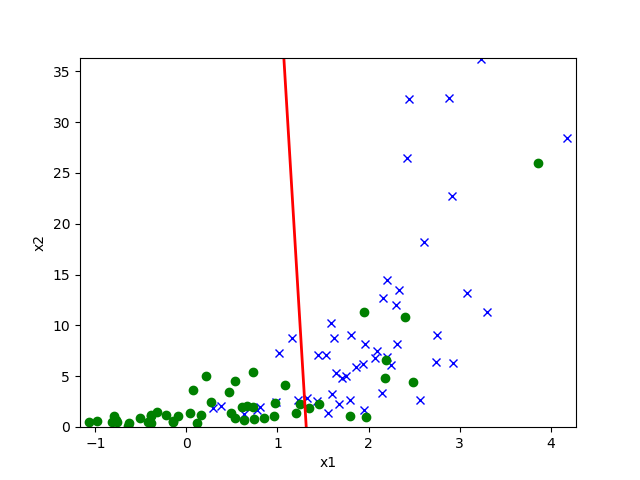
\includegraphics[width=0.65\linewidth]{01-linearclass/p01e_pred_1.png}
    \caption{Separating hyperplane for GDA on the validation set for Dataset 1 (Note: This is for reference only.  You are not required to submit a plot.)}
\end{figure}

	\item \points{1f}
For Dataset 1, compare the validation set plots obtained in part (b) and part (e)
from logistic regression and GDA respectively, and briefly comment on your observation in a couple of lines. No plot submission is required.

	\item \points{1g}
Use autograder test case |1g-0-basic| to create GDA and logistic regression plots for Dataset 2. Compare the plots for Dataset 1 (from parts (b) and (e)) with the plots for Dataset 2.  On which dataset does GDA seem to perform worse than logistic regression? Why might this be the case?

	\item \points{1h} For the dataset where GDA performed worse in parts (f) and (g), can you find a transformation of the $x^{(i)}$'s such that GDA performs significantly better? What might this transformation be?

\end{enumerate}
